%# -*- coding: utf-8-unix -*-
% !TEX program = xelatex
% !TEX root = ../thesis.tex
% !TEX encoding = UTF-8 Unicode
%%==================================================
%% chapter01.tex for SJTU Master Thesis
%%第一章
%%==================================================
\chapter{绪论}
\section{课题背景及研究意义}
\subsection{课题研究背景}
人工智能(Artificial Intelligence,AI)是研究、开发用于模拟延伸和扩展人的认知,识别,分析和决策的多种功能的一门新兴科学技术,其涵盖了统计学,计算机科学,脑神经科学和社会科学等学科。人工智能的应用领域包括语音识别,机器人,图像识别,自然语言处理和专家系统等等。在90年代,"深蓝" 计算机与卡斯帕罗夫决战,"深蓝"获胜,公众再次把注意力放在了人工智能,2016年,谷歌的AlphaGo赢了韩国棋手李世石,引发人工智能热潮,2018年腾讯人工智能实验室推出的“绝艺”在腾讯世界人工智能围棋大赛决赛中以7:0的比分战胜星战围棋\cite{人工智能产业形势分析课题组20182018},这些都代表了特定时期人工智能发展的技术水平。人工智能的实现算法在现代被称为机器学习,根据机器学习的应用数据和模型任务,可以分成监督学习,无监督学习和强化学习。本文研究的深度强化学习是在强化学习的框架下使用了深度学习作为奖励函数拟合的工具,下面分别介绍传统的强化学习和深度学习概念。

深度学习是利用多层的神经网络建立更加复杂的模型,对数据有更深刻全面的理解。深度学习网络把原始数据通过简单的非线性函数进行映射,转换为高层次抽象的表达,通过加大神经网络的深度进行多次非线性映射堆叠,可以表示出非常复杂的模型。通过在学习过程中引入紧缩性和鲁棒性的约束,网络后端的特征输出部分不仅可以强化对输入数据的区分和预测能力,同时可以避免外界噪声和其他不相关因素的干扰。因此在浅层网络无法全面客观表示数据特征,学习数据分布的时候可以采用深度学习网络进行统一的特征学习框架的搭建。深度学习各层的输入特征不是根据具体任务人为处理的,而是利用一种通用的映射和优化的过程从原始数据中学习得到。特征提取工作和分类预测任务被深度学习框架进行统一整合,避免了繁琐的人类手工设计提取特征的过程,实现了端到端的自动学习。准确的说深度学习首先利用无监督学习对每一层的网络节点进行预训练学习模型,并将当前层的输出数据作为输入数据传入给下一层,最后一层采用监督学习方式,根据网络的最后一层输出结果进行前向传播进行网络参数的整体微调优化。经过若干次的参数迭代可以得到相对稳定的网络结构。

伴随着AlphaGo的诞生,强化学习(Reinforcement Learning)作为其核心算法逐渐成为机器学习研究的另一大热点。有学者认为,智能系统必须能够在不接受持续监督的情况下自主学习,而强化学习正是其中的最佳代表。一个AI系统必须能够自己判断对错,只有这样才能扩展到大量的知识和一般技能。学习一个好的,而非新的表征对于解决大多数现实世界中的问题来说具有至关重要的作用。这些表征通常不需要被显式地描述,而是可以通过内部奖励机制来进行引导,强化学习就是这样一种学习方式。强化学习理论的发展受到生理学、神经科学和最优控制等领域的启发,在控制理论、机器人学、运筹学、经济学等领域内部,同样有很多的学者投身强化学习的研究。追随强化学习的发展历史,从1956年提出的动态规划方法,到1977年提出的自适应动态规划算法以及1988年的时间差分算法,1922年Q-learning算法首次被提出,后来又衍生出很多改进的强化学习算法,包括Saras算法,置信上限树算法,确定性策略梯度算法,等等。强化学习被广泛应用在仿真模拟\cite{傅启明2014一种基于线性函数逼近的离策略}、工业制造\cite{高阳2007平均奖赏强化学习算法研究}、优化与调度\cite{魏英姿2005一种基于强化学习的作业车间动态调度方法},机器人控制\cite{Ipek2008Self}、游戏博弈\cite{Tesauro1944TD}等领域。

强化学习是获得最大累积奖励的决策过程。因此相比于其他机器学习算法,强化学习更加注重学习解决问题的策略。如何建立最优的状态动作映射关系(map situations to actions)是强化学习要解决的核心问题,在时间延迟的监督信息下,强化学习需要通过大量的尝试探索出适合当前场景的最优策略。

\subsection{课题研究意义}
早期的强化学习需要人为干预特征的提取,然而人类的认知并不一定是全面且完备的,同时人工提取特征进行标注需要消耗大量的资源。受深度学习提取特征的启发,通过深度学习网络代替手工设计或领域启发式算法进行前期的特征提取工作,智能体直接从原始输入构建和获取自己的知识库,增强了强化学习的特征学习能力。这种结合深度学习进行特征构建和函数拟合的强化学习算法称为深度强化学习。深度强化学习结合了深度学习较强的感知能力和传统强化学习优秀的决策能力,通过端对端的学习方式实现了组合策略,做到了对原始数据从输入到输出的直接控制。其算法的整体框架如图\ref{fig:DRL}所示。
\begin{figure}[htbp]
	\centering
	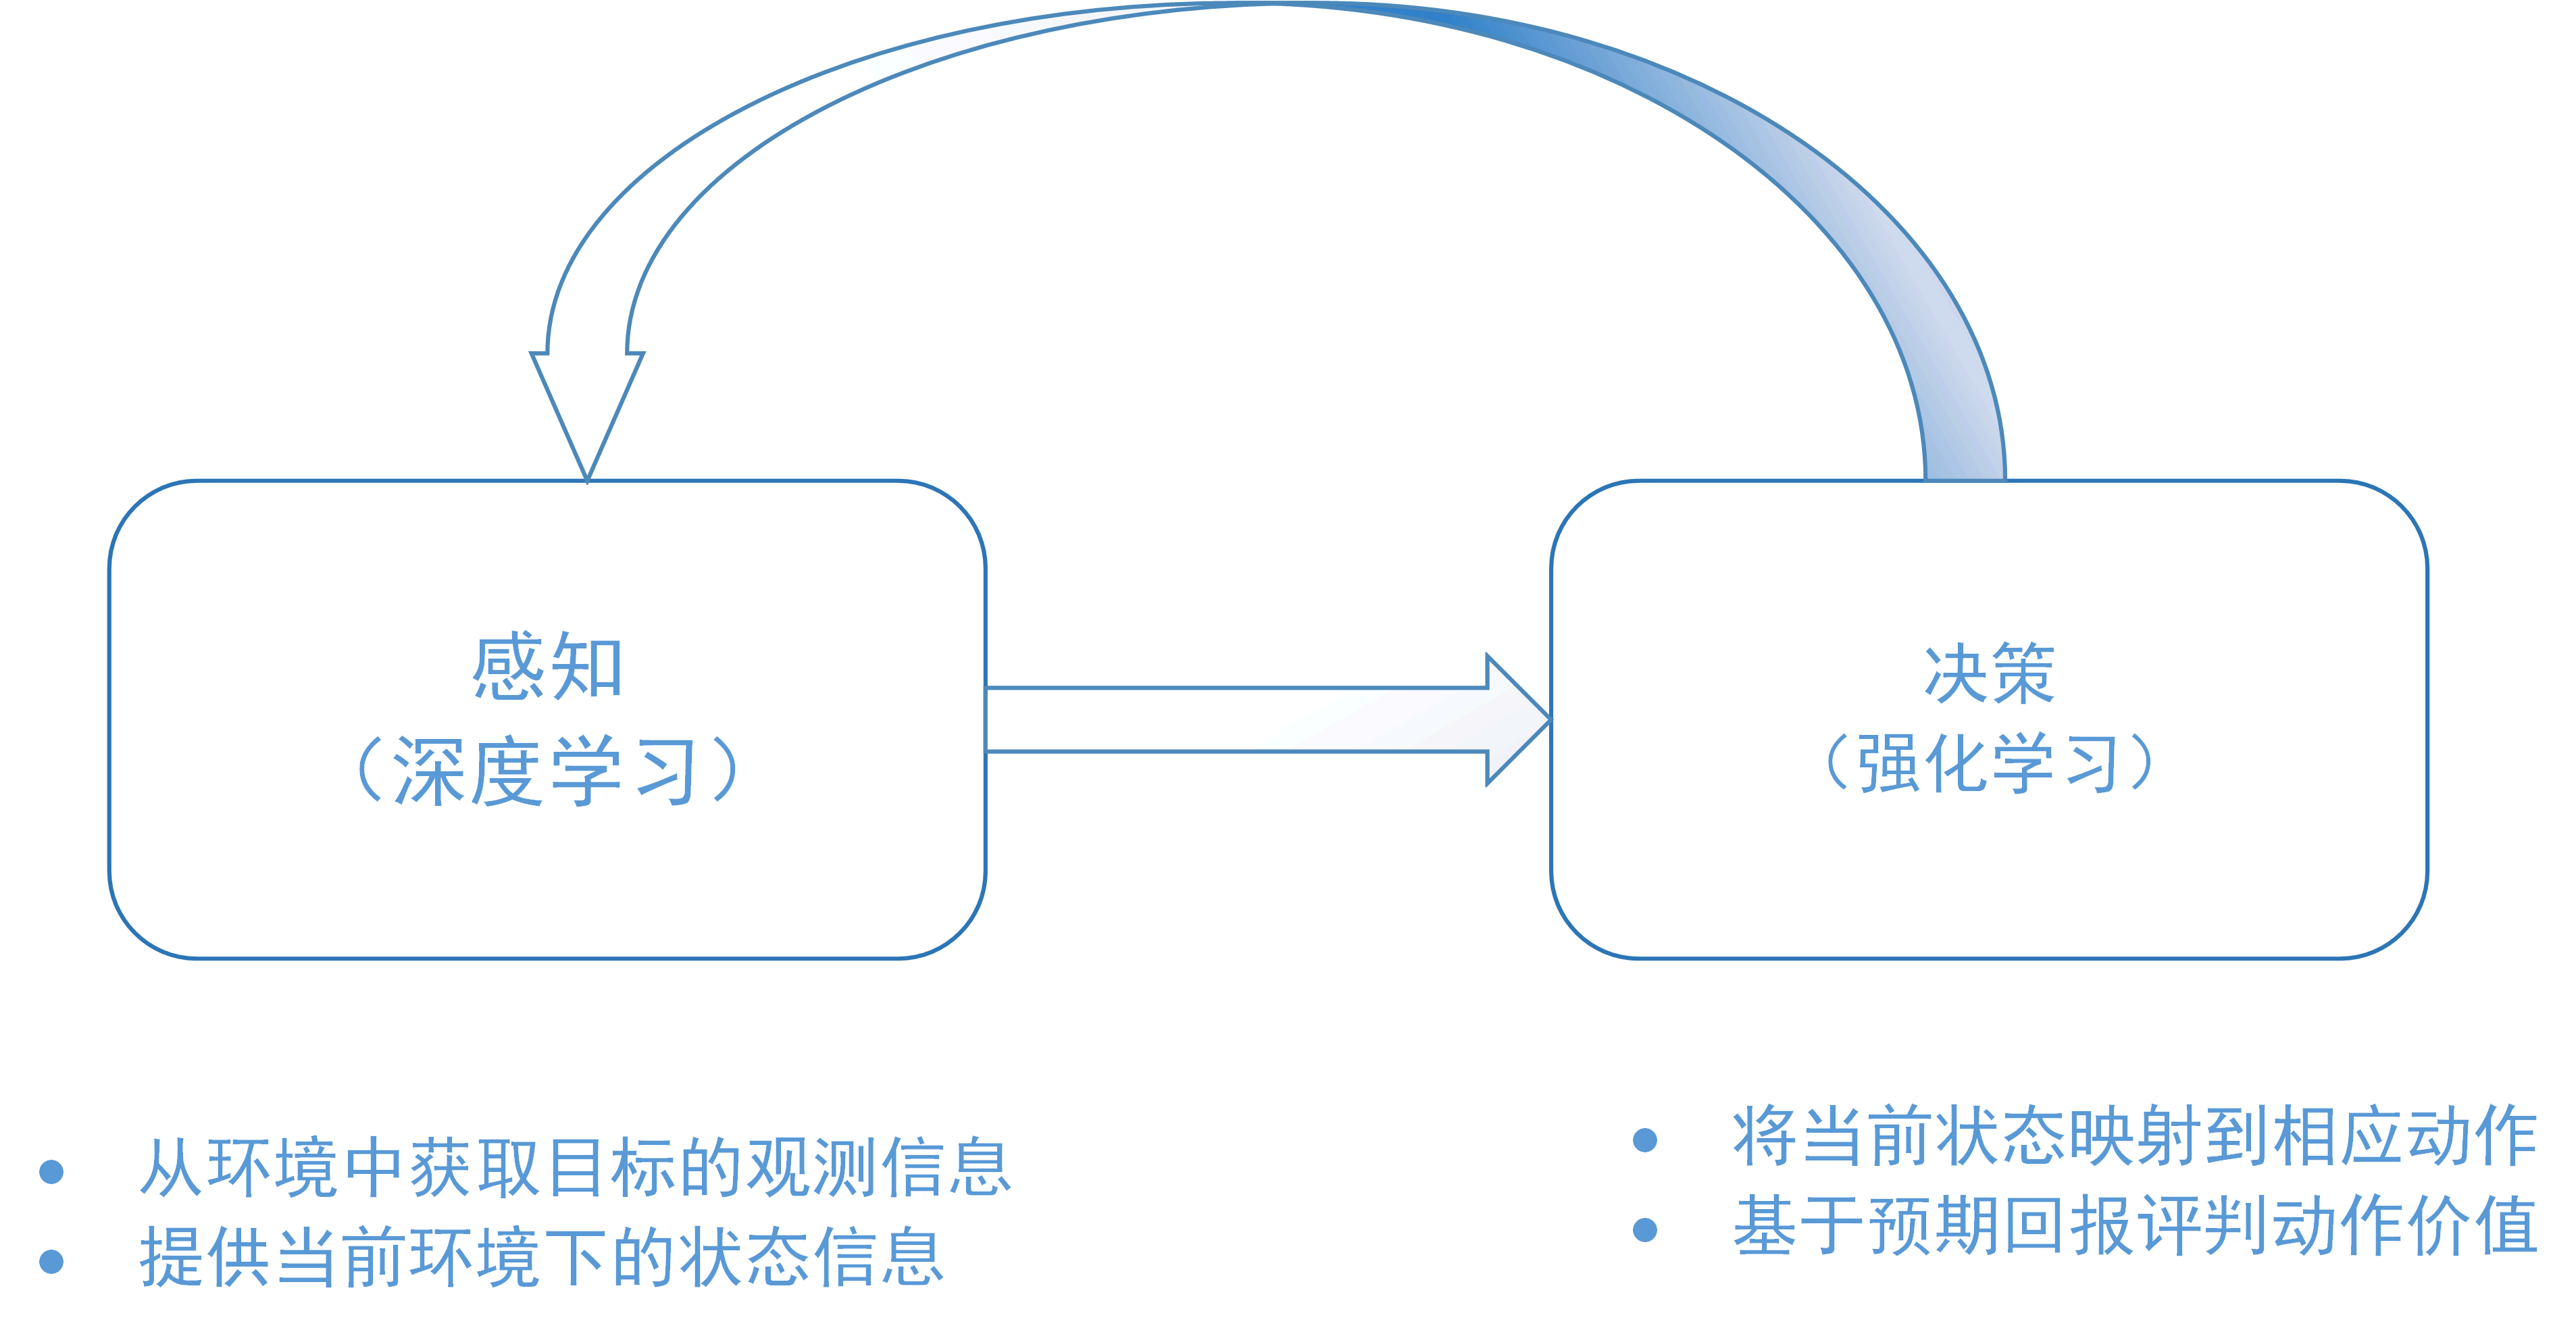
\includegraphics[width=\hsize]{example/DRL.png}
	\bicaption[深度强化学习框架]
	{深度强化学习框架}
	{The fremework of deep reinforcement learning}
	\label{fig:DRL}
\end{figure}

近年来深度强化学习在以惊人的速度发展,各个团队相继在探索强化学习在不同领域的新方法和新应用。其进步的速度是有目共睹的,在不到两年的时间里,深度强化学习衍生了很多新算法,如:深度Q网络(Deep Q Network,DQN)\cite{Roderick2017Implementing}, AlphaGo\cite{Silver2016Mastering},以及可微分神经计算机\cite{Graves2016Hybrid},在应用上,决斗网络(dueling network)架构\cite{Wang2015Dueling},ACL上的口语对话系统\cite{Su2016On},EMNLP上的信息提取\cite{Narasimhan2016Improving},以及 NIPS上的价值迭代网络(value iteration networks)\cite{Tamar2017Value},异步方法\cite{Mnih2016Asynchronous},用于机器翻译的双学习(dual learning)\cite{Xia2016Dual},生成对抗式模仿学习\cite{Ho2016Generative},无监督强化和辅助学习\cite{Jaderberg2016Reinforcement},神经架构设计\cite{Pham2018Efficient}等等。新的学习机制也在出现,例如把强化学习和无监督,半监督,迁移学习结合提升学习的质量和速度。新的强化学习算法还在不断涌现,学习模型会带来稳定性,收敛性,数据效率,可扩展性,速度,简洁性,可解释性,稳健性和安全性的问题,奖励反馈机制的建立也是很重要的一环,奖励可能来自认知科学领域,涉及物理学,因果模型,组合性学习等各个领域的知识。强化学习作为一种更为通用的学习和决策范式,将会给深度学习、机器学习和广义上的人工智能带来深远的影响。

\section{深度强化学习国内外研究现状}
在高级人工智能领域,感知和决策都是衡量智能的重要指标。强化学习在理论和算法层面已经取得了一系列的成就,将深度学习和强化学习结合起来,优势互补,为复杂系统的感知与决策问题提供了有效的解决思路。国内外关于深度强学习的研究成果层出不穷。

\subsection{深度强化学习国外研究成果}
深度强化学习研究的初期思路就是利用神经网络完成数据的降维任务,将较高维度的特征经过神经网络变换到较低维度,降低强化学习处理的难度。典型的应用包括利用神经网络提取视觉信号的输入,控制机器人推箱子\cite{Shibata2003Acquisition},将强化学习和深层自动编码机结合,利用“视觉动作学习”完善智能体的感知能力\cite{Lange2010Deep},将深度置信网络代替传统的值函数逼近器,用于车牌字符分割识别\cite{Abtahi2015A},深度拟合Q学习利用视觉输入信号结合深度强化学习框架用于车辆控制的问题。同时期实现视频赛车自动驾驶策略规划的还有利用神经演化方法(neural evolution, NE)和强化学习进行结合\cite{Kumar2014Understanding}。

受上述前期工作的启发,很多学者开始将卷积神经网络和强化学习算法进行感知和决策图像数据任务。深度Q网络(deep Q network, DQN)\cite{Mnih2013Playing}在2013年被深智团队首次提出,其思想是将CNN网络和Q学习进行结合,利用经验回放技术优化网络。DQN网络是深度强化学习领域的突破,其输入数据是原始游戏画面,输出状态动作Q函数,实现了端到端的学习控制。DQN网络的出现引发了深度强化学习的热潮,众多学者提出了很多改进方案,如深度Q网络\cite{Schaul2015Prioritized},通过对历史数据进行先后顺序排序,提高重要数据采样比例。Nair等提出了深度Q网络的大规模分布式架构Gorila\cite{Goeringer2013Massively}解决了网络训练过程缓慢的问题。Guo等首次将蒙特卡洛搜索树和原始深度Q网络结合\cite{Guo2014Deep},用于实时处理Atari游戏,效果好于原始深度Q网络。将两个Q学习网络运用到深度Q网络中的双重深度Q网络(double-DQN)\cite{DQN}解决了原始Q网络中对由于固有估计误差造成的过高估计动作值函数的的问题。为了加快强化学习的训练速率,Mnih等改进了异步深度强化学习方法\cite{Mnih2016Asynchronous}。
\subsection{深度强化学习国内研究成果}
中国的技术公司并不示弱,阿里、腾讯、百度、滴滴和天壤等国内团队将深度强化学习应用到搜索、推荐、营销、派单和路径规划等实际问题的决策任务中,同时在无人驾驶方向进行了探索。2018年阿里发行了第一本人工智能强化学习电子书《从虚拟世界走进现实应用——强化学习在阿里的技术演进与业务创新》,平台作为信息的载体,需要在与消费者的互动过程中,根据对消费者(环境)的理解,及时调整 提供信息(商品、客服机器的回答、路径选择等)的策略,从最化过程累积收益(消费者在平台上的使体验)。基于监督学习式的信息提供段,缺少有效的探索能力,系统倾向于给消费者推送曾经发过为的信息单元(商品、店铺或问题答案)。强化学习作为种有效的基于户与系统交互过程建模和最化过程累积收益的学习法,在某些具体的业务场景中进了很好的实践并得到大规模应。从2016年起,腾讯AILab开始研发围棋人工智能程序,于2017年分别在“AI龙星战”和“UEC杯”等世界计算机围棋大赛上斩获冠军,2018年加强版的围棋智能程序“绝艺”问世,首次在让子棋中战胜顶级职业棋手柯洁九段和连笑九段。让子棋是人类通过人工智能不断探索围棋边界的典型范例。百度也相继提出把强化学习应用在信息流质量的提升中,利用强化学习识别移除标题党,并在凤巢广告系统里部署了强化学习系统,充分利用了强化学习不需要数据标注,可以有效利用更多数据信息,能实现在线学习等优点。在强化学习模型中,广告的优化行为是通过广告投放系统的所带来的奖励,观察广告竞价状态实现的。
深度强化学习通过不断的进步和发展, 在理论与应用层面取得了长足的进步。 表格\ref{tab:1}总结了深度强化学习发展历程中的重要事件。
\begin{table}[htpb]
	\centering
	\bicaption[深度强化学习研究历程]
	{深度强化学习研究历程}
	{Timeline of deep reinforcement learning research events.}
	\label{tab:1}
	\begin{tabular}{ll}
		年份 & 事件 \\ \midrule
		2013 & Mnih 等提出了深度强化学习的开创性工作DQN在视频游戏领域取得突破 \\
		2014& Guo 等提出DQN与MCTS结合的算法 \\
		2015 &Van 等提出了双重深度Q网络(double-DQN) \\
		2015&Hausknecht等结合LSTM提出了深度递归Q网络(DRQN)\\
		2015&Sorokin等结合注意力网络提出了深度注意力递归Q网络(DARQN)\\
		2016&深智团队在《Nature》上面发表了基于DRL的计算机围棋程序-Alphago\\
		2017&深智团队改进AlphaZero问世\\
		2018&腾讯AI LAb的“绝艺”斩获冠军\\
		 \bottomrule
	\end{tabular}
\end{table}
\subsection{现有研究不足和展望}
尽管随着深度强化学习的不断发展,越来越多的实际问题得到了有效的解决,深度强化学习在理论方面和应用方面仍然存在很多不足之处,如何有效解决这些缺点并拓展强化学习的应用场景将成为以后研究的重点方向。不足包括:
\begin{enumerate}
	\item 当强化学习智能体的动作具体到生成数据时变成了生成式对抗网络(Generative Adversarial Networks,GAN),现有的生成式对抗网络模型大多数应用于图像视频数据的生成任务上,应用于非图像类数值数据的场景比较少,同时存在模式崩溃,生成样本数据分布覆盖不足的缺点。
	\item 深度强化学习的另一个主要应用于Atari视频游戏的自主决策,在这里的奖励是通过不断和游戏环境进行交互得到的。在其他应用场景奖励函数的选择和设计显得尤为重要。深度强化学习模型的泛化能力较弱,对于某些场景下表现效果好的模型不一定适用于其他场景。所以模型效果也直接依赖于环境的搭建。
	\item 目前强化学习解决实际问题中最成功的应用是与蒙特卡罗树搜索结合的方法进行一对一智能体两人零和完全信息博弈。多智能体博弈,包括零和,非零和,完全信息,不完全信息博弈的问题都需要进一步研究和扩展。机器学习算法的前提是数据在相同的特征空间具有相同的数据分布,但是现实环境的模型是比较复杂的,这种强制假设限制了深度强化学习的应用范围。
	\item 深度强化学习奖励反馈机制的建立是又一大难题,在部分应用场景反馈可以是确定性函数,但是大部分的应用场景反馈来自和环境的交互,所以需要把深度强化学习知识和其他学科进行结合,包括心理学,数据科学,计算机科学,神经网络感知科学,等等。
	\item 虽然深度强化学习有广阔的应用前景有待挖掘,但是很多应用者对于其理论层面的研究还不够深入,目前为止深度强化学习相关的文章并没有给出其学习过程收敛性的证明,只能通过是实验结果观察模型的学习效果。对模型的准确认知对于模型的完善和应用是非常关键的。从长远发展来看,理论基础的夯实会利于深度强化学习的良性发展。
\end{enumerate}
\section{主要内容与章节安排}
\subsection{本文的主要工作和创新点}
针对深度强化学习和博弈模型结合的应用现状,本文的创新点如下:
\begin{enumerate}
	\item 具体化强化学习任务,利用GAN生成式对抗网络对小数据集进行扩充,并在现有WGAN网络的基础上引入监督信息,完善学习数据分布信息。
	\item 利用self-paly方式不依赖于人类专家数据进行智能体博弈仿真数据生成,根据相对熵自适应调整学习率加快深度学习网络收敛,结合$softmax$和$\varepsilon$贪心策略解决强化学习中探索和利用平衡的问题,并以五子棋为例进行实验效果分析。
	\item 把深度强化学习应用于飞机对战场景,由一对一智能体对抗拓展到多智能体之间的对抗和合作,进行奖励的自动分配和对战策略的学习,设计实验场景并进行实验分析。
\end{enumerate}
\subsection{本文的内容安排}
本文主要研究深度强化学习在对抗类博弈策略上的应用。通过对不同强化学习模型的研究和对比,本文实现了基于GAN生成式对抗网络的数据扩充和预测,利用AC模型的单智能体一对一仿真,和针对空战问题的二对二策略仿真。
具体的研究内容和章节安排如下:

第一章 介绍了本课题的背景及研究意义,指出存在的技术难点,介绍了目前国内外深度强化学习的研究概况。

第二章主要介绍了传统的强化学习的种类和基本原理,以及结合深度学习模型改进之后的强化学习模型的各种变体原理及相关应用。并结合Alphago以及Alphazero的实现过程剖析背后的主要技术。

第三章针对小样本本缺失数据扩充的具体问题,对不同数据集进行扩充,包括电子设备参数数据的扩充以及不同股票收盘指数数据,由于GAN网络应用场景主要是图像数据,在本章节提出针对数值类数据的改进的引入监督信息的GAN生成式对抗网络对数据进行扩充和预测,利用实验结果分析模型的收敛性以及数据扩充效果。

第四章针对棋盘类游戏零和博弈的问题,提出了类比Alphazero原理的的无先验数据进行训练的Actor-Critic强化学习模型,针对深度学习网络收敛慢的问题引入了基于相对熵的自适应学习率,针对强化学习探索利用平衡的问题引入了噪声系数,以五子棋为实验场景,根据最后人机博弈和智能体自我博弈作战的策略以及训练的损失函数曲线进行分析。改进的算法收敛更快,模型策略更优。

第五章针对飞机作战场景,设计飞机一对一作战,根据结果分析场景迁移的可行性,在此基础上设计二对二多智能体竞争合作结合的应用场景,通过深度强化学习实现根据作战规则和最终奖励的分配实现队间飞机和队内飞机奖励的自动分配,根据人机对弈过程分析策略合理性,证明模型的可行性。

第六章总结以上核心章节的研究内容和创新点,并对针对现有研究工作的不足提出今后的研究展望。
